\documentclass[a4paper, 11pt]{article}
\usepackage{comment} % enables the use of multi-line comments (\ifx \fi) 
\usepackage{lipsum} %This package just generates Lorem Ipsum filler text. 
\usepackage{fullpage} % changes the margin
\usepackage{graphicx}
\usepackage{epsfig}
\usepackage{listings}
\usepackage{xcolor}
\lstset { %
	language=C++,
	backgroundcolor=\color{black!5}, % set backgroundcolor
	basicstyle=\footnotesize,% basic font setting
}

\begin{document}
%Header-Make sure you update this information!!!!
\noindent
\large\textbf{Lab 2 Report} \hfill \textbf{Abhishek Srivastava} \\
\normalsize CS260-001: Computer Security \hfill Student Id: 861307778 \\
\normalsize Prof. Heng Yin \hfill 30/Jan/2017 \\
\hrule

\section*{Problem : Implementing a pintool for shadow stack}
Objective for this lab assignment is to implement a shadow stack through dynamic binary instrumentation using Pin.

\section*{Solution}
Shadow stack is a well-known and effective defense mechanism to defeat control-flow hijacking attacks that aim to overwrite a return address on the stack. The general algorithm works like : For each “call” instruction, identify the return address, and push it onto the shadow stack. For each “ret” instruction, identify the return target and see if it matches with the value on the top of the shadow stack. If so, pop up the value from the shadow stack otherwise, report an attack.

In Figure 1 you can see the Trace implementation of detecting the instruction to be of calling or returning type. We are going from block to block and for each tail instruction we are checking that whether it is calling or returning instruction. Iterating over blocks and checking only tail instructions makes this process fast by not going over each instructions. After checking we are executing based on the type of instruction, If it is a calling instruction we are passing it to the \textbf{do\_call} analysis section or if it is returning instruction we are passing it to the \textbf{do\_ret} analysis section.

In the Figure 2 you can see the implementation of both \textbf{do\_call} and \textbf{do\_ret} analysis section. In \textbf{do\_call} section I am pushing the return address (\textbf{IARG\_RETURN\_IP}) parameter to the stack called \emph{shadow}. In \textbf{do\_ret} analysis section I am checking whether the top of \emph{shadow} stack is same as the returning address(\textbf{IARG\_BRANCH\_TARGET\_ADDR}). If they are the same value then it is okay to proceed and buffer overflow exploit has not been used. I am also maintaining a global parameter \textbf{isOkay} which can extended to stop the further execution. If the addresses are not same I am printing the error and setting \textbf{isOkay} to false because return address has been changed by buffer overflow exploit.

Figure 3, 4 and 5 are the executions of compiled code. In Figure 2 \& 3, I tested the implementation by calling \textbf{/bin/ls} and \textbf{/bin/ps} whose output did not raised any error and produced the correct expected output. In Figure 5, I did 3 tests, First I checked whether code is giving Access denied message when the input is wrong password, then I checked if Access Granted is showed when inputed with correct password and at last I tested by overflowing the input buffer. Which as expected printing Error message that stack values does not match and segmentation fault is occurring which can be prevented using \textbf{isOkay} variable but I have not implemented it as it was not required.

Another thing which can be extended as well is maintaining shadow stacks for multi-threaded system. 
\textbf{IARG\_THREAD\_ID} can be used to maintain a global dictionary which can then be mapped to a particular shadow stack which will maintain the return address for that particular thread and rest of the implementation is same as for a single threaded system.   

\begin{figure}
	\centering
	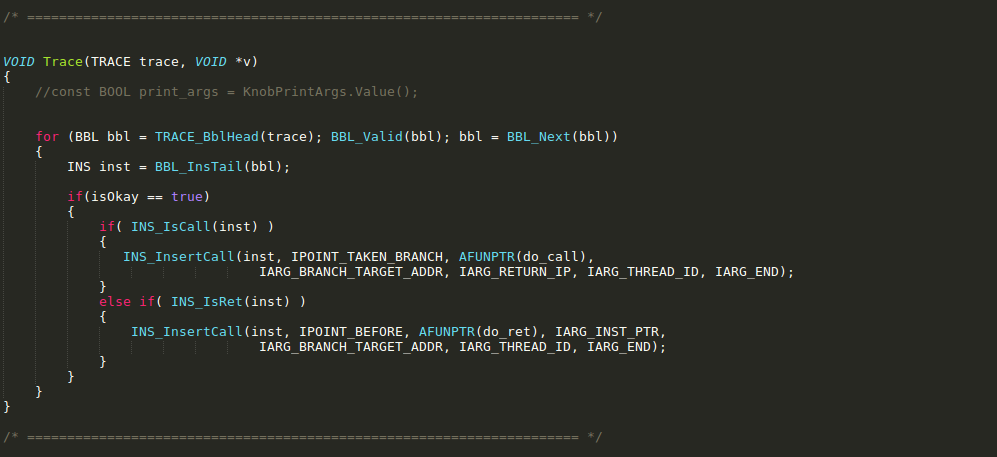
\epsfig{file=Lab_2_ss_5.png, height=4in, width=7in}
	\caption{TRACE section implementation.}
\end{figure}
\begin{figure}
	\centering
	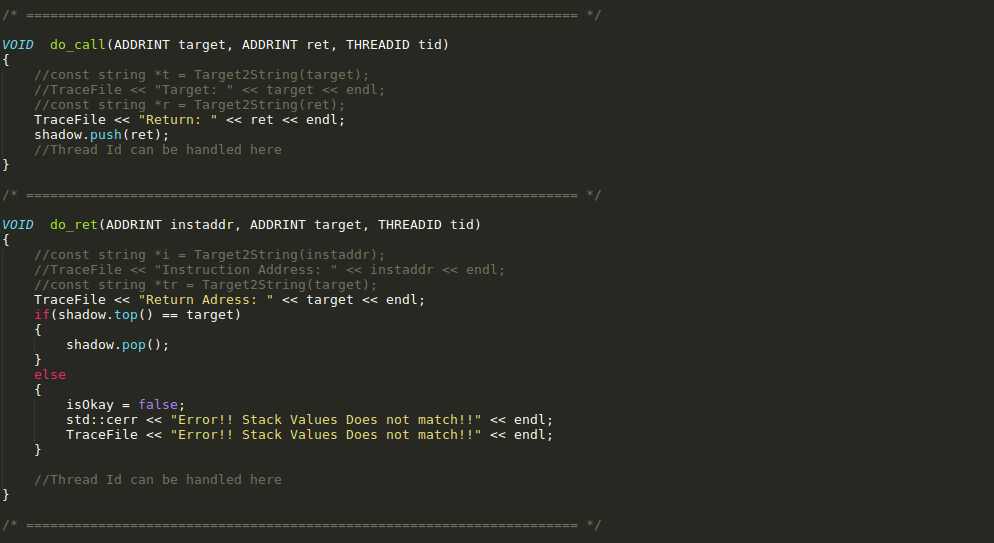
\epsfig{file=Lab_2_ss_4.png, height=4in, width=7in}
	\caption{do\_call and do\_ret analysis section implementation.}
\end{figure}
\begin{figure}
	\centering
	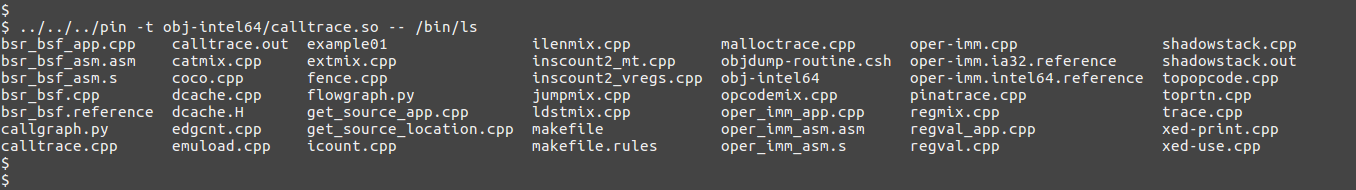
\epsfig{file=Lab_2_ss_1.png, height=1.5in, width=7in}
	\caption{Output of /bin/ls test with compiled code.}
\end{figure}
\begin{figure}
	\centering
	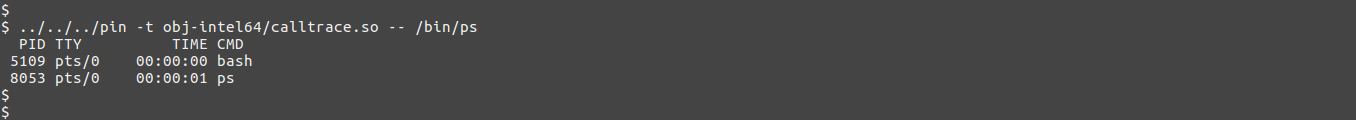
\epsfig{file=Lab_2_ss_2.png, height=1in, width=7in}
	\caption{Output of /bin/ps test with compiled code.}
\end{figure}
\begin{figure}
	\centering
	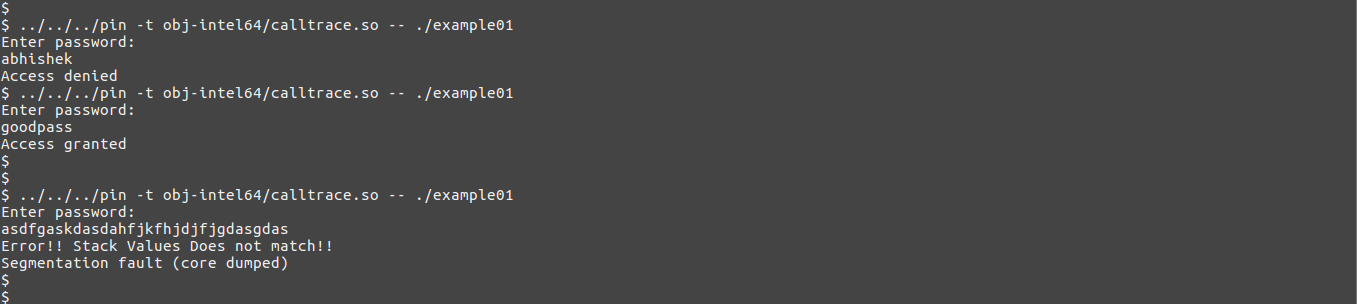
\epsfig{file=Lab_2_ss_3.png, height=2in, width=7in}
	\caption{Outputs of normal and buffer overflow exploit testing.}
\end{figure}
\newpage
\section*{Code Implementation of shadow stack}
\begin{lstlisting}

#include ``pin.H''
#include <iostream>
#include <fstream>
#include <stack>
/* ===================================================================== */
/* Global Variables                                                      */
/* ===================================================================== */
std::ofstream TraceFile;
std::stack<ADDRINT> shadow;
static bool isOkay = true;
/* ===================================================================== */
/* Commandline Switches                                                  */
/* ===================================================================== */
KNOB<string> KnobOutputFile(KNOB_MODE_WRITEONCE, ``pintool'', ``o'',
                            ``shadowstack.out'', ``specify trace file name'');
/* ===================================================================== */
/* Print Help Message                                                    */
/* ===================================================================== */
INT32 Usage()
{
    cerr << ``This tool produces a call trace.'' << endl << endl;
    cerr << KNOB_BASE::StringKnobSummary() << endl;
    return -1;
}
string invalid = ``invalid_rtn'';
/* ===================================================================== */
/* Handling if instruction is of INS_IsCall type.                        */
/* ===================================================================== */
VOID  do_call(ADDRINT target, ADDRINT ret, THREADID tid)
{
    //Writing to the TraceFile
    TraceFile << ``Return: '' << ret << endl;
    //Pushing the ret(IARG_RETURN_IP) to the stack
    shadow.push(ret);
}
/* ===================================================================== */
/* Handling if instruction is of INS_Ret type.                           */
/* ===================================================================== */
VOID  do_ret(ADDRINT instaddr, ADDRINT target, THREADID tid)
{
    //Writing to the TraceFile
    TraceFile << ``Return Adress: '' << target << endl;
    //Checking if the top of stack is same as target(IARG_BRANCH_TARGET_ADDR).
    if(shadow.top() == target)
    {
        //If they are the same pop the return address
        shadow.pop();
    }
    else
    {
        //If they are not same set isOkay as false and print the error and 
        //write it to the TraceFile
        isOkay = false;
        std::cerr << ``Error!! Stack Values Does not match!!'' << endl;
        TraceFile << ``Error!! Stack Values Does not match!!'' << endl;
    }  
}
/* ===================================================================== */
/* Trace Instrumentation Implementation.                                 */
/* ===================================================================== */
VOID Trace(TRACE trace, VOID *v)
{
    //Iterating over blocks
    for(BBL bbl = TRACE_BblHead(trace); BBL_Valid(bbl); bbl = BBL_Next(bbl))
    {
        //Getting the tail instruction
        INS inst = BBL_InsTail(bbl);
        //If isOkay is true
        if(isOkay == true)
        {
            //Checking if the instruction is INS_InCall type or INS_Ret type
            if( INS_IsCall(inst) )
            {
                //calling do_call analysis section
                INS_InsertCall(inst,IPOINT_TAKEN_BRANCH,AFUNPTR(do_call),
                  IARG_BRANCH_TARGET_ADDR,IARG_RETURN_IP,IARG_THREAD_ID,IARG_END);     
            }
            else if( INS_IsRet(inst) )
            {
                //calling do_ret analysis section
                INS_InsertCall(inst,IPOINT_BEFORE,AFUNPTR(do_ret),IARG_INST_PTR,
                        IARG_BRANCH_TARGET_ADDR,IARG_THREAD_ID,IARG_END);
            }
        }
    }
}
/* ===================================================================== */
VOID Fini(INT32 code, VOID *v)
{
    TraceFile << ``# eof'' << endl;
    TraceFile.close();
}
/* ===================================================================== */
/* Main                                                                  */
/* ===================================================================== */
int  main(int argc, char *argv[])
{

    PIN_InitSymbols();

    if( PIN_Init(argc,argv) )
    {
        return Usage();
    }
    TraceFile.open(KnobOutputFile.Value().c_str());
    TraceFile << hex;
    TraceFile.setf(ios::showbase);
    string trace_header = string(``#\n''
                                 ``# Call Trace Generated By Pin\n''
                                 ``#\n'');
    TraceFile.write(trace_header.c_str(),trace_header.size());
    TRACE_AddInstrumentFunction(Trace, 0);
    PIN_AddFiniFunction(Fini, 0);
    // Never returns
    PIN_StartProgram();
    return 0;
}
\end{lstlisting}
\end{document}
